\documentclass{article}
\usepackage[utf8]{inputenc}
\usepackage{amsmath}
\usepackage{amsthm}
\usepackage{amsfonts}
\usepackage{amssymb}
\usepackage{amstext}
\usepackage{gensymb}
\usepackage{graphicx}
\usepackage{enumerate}
\pagenumbering{arabic}
\usepackage{fancyhdr}
\usepackage[margin=0.75in]{geometry}
\usepackage{eucal}
\usepackage{parskip} % removes auto indentation for paragraphs
\usepackage{enumitem} % changes the indexing for enumerate
\setlist[enumerate,1]{label = {(\alph*)}}

\usepackage{listings} % import code into latex

\usepackage{subcaption}

\def\N{\mathbb{N}}
\def\Z{\mathbb{Z}}
\def\Q{\mathbb{Q}}
\def\R{\mathbb{R}}
\def\C{\mathbb{C}}
\newcommand{\Mod}[1]{\ (\text{mod}\ #1)}
\newcommand{\Problem}[1]{\textbf{Problem #1}}
\newcommand{\li}[0]{\liminf_{n\to\infty}}
\newcommand{\ls}[0]{\limsup_{n\to\infty}}
\newcommand{\dl}[2]{\displaystyle\lim_{#1 \to #2}}
\newcommand{\ds}[2]{\displaystyle\sum_{#1}^{#2}}
\newcommand{\ra}{\Rightarrow}

\linespread{1.5}

\usepackage{float}

\pagestyle{fancy}
\fancyhf{}
\rhead{CSE 6643}
\lhead{Alexander Winkles}
\chead{\Large \textbf{Homework 1}}
\cfoot{Page \thepage}

\begin{document}

\Problem{1}

Suppose $A$ is a lower triangular matrix. 
Let $I$ be the identity matrix. 
We wish to show that $A^{-1}$ is also lower triangular. 
Notice that $I = AA^{-1}$. 
Let $a_{ij}$ and $b_{ij}$ be the elements of $A$ and $A^{-1}$ respectively. 
Then we can establish the following relationship:
\begin{equation*}
\begin{cases}
    a_{11}b_{1j} = \delta_{1j}\\
    a_{21}b_{1j} + a_{22}b_{2j} = \delta_{2j}\\
    \vdots\\
    a_{n1}b_{1j} + \hdots + a_{nn}b_{nj} = \delta_{nj}\\
\end{cases}
\end{equation*}
where $\delta_{ij}$ is the Kronecker Delta.
This may be rewritten as follows:
\begin{equation*}
\begin{cases}
    b_{1j} = \frac{\delta_{1j}}{a_{11}} \\
    b_{2j} = \frac{\delta_{2j} - a_{21}b_{1j}}{a_{22}} \\
    \vdots \\
    b_{nj} = \frac{\delta_{nj} - \sum_{k=1}^{n-1} a_{nk}b_{kj}}{a_{nn}}\\
\end{cases}
\end{equation*}
Thus it can be seen that whenever the column index exceeds the row index for $b_{ij}$, $b_{ij} = 0$, so $A^{-1}$ is lower triangular. 
$\square$

\Problem{2}

Let $||A||$ be an induced matrix on some $A \in \C^{m*m}$.
By definition, $\rho(A) = \lambda_{\text{max}}$.
Consider the eigenvector for $\lambda_{\text{max}}$, $x$.
By definition, $Ax = \lambda_{\text{max}}x$.
Taking their norms gives $||Ax|| = ||\lambda_{\text{max}}x|| = |\lambda_{\text{max}}||x|$.
This can be rewritten as $||A|| |x| \geq |\lambda_{\text{max}} |x|$, then removing $|x|$ gives $||A|| \geq |\lambda_{\text{max}} = \rho(A)$ as desired.
$\square$

\Problem{3}

Suppose $A \in \C^{202*202}$ with $||A||_2 = 100$ and $||A||_F = 101$.
From the text, we know $||A||_2 = \sigma_1$ and $||A||_F = \sqrt{\sigma_1^2 + \hdots + \sigma_n^2}$.
Thus, $101 = \sqrt{10000 + \hdots + \sigma_{202}^2}$ after plugging in values.
Rearranging, this becomes $201 = \sigma_2^2 + \hdots + \sigma_{202}^2$.
Since the smallest value $\sigma_{202}$ can obtain is 1, we arrive at $\sigma_1/\sigma_{202} \geq 100$. 

\Problem{4}

For this problem, I implemented a code ``Problem4'' in MATLAB that generated random matrices of size $m*m$ with a mean value of $0$ and a standard deviation of $\sqrt{m}$. 
Using MATLAB's built-in norm functions, I obtained the p-norm for p$=1,2,\infty$ for the random matrices. 
As my GTID is odd, I computed the ratio between the 2-norm and infinity-norm as well. 
Additionally, I computed the average condition number for the matrices.
My results are shown below:

\begin{figure}[H] % "[t!]" placement specifier just for this example
\begin{subfigure}{0.48\textwidth}
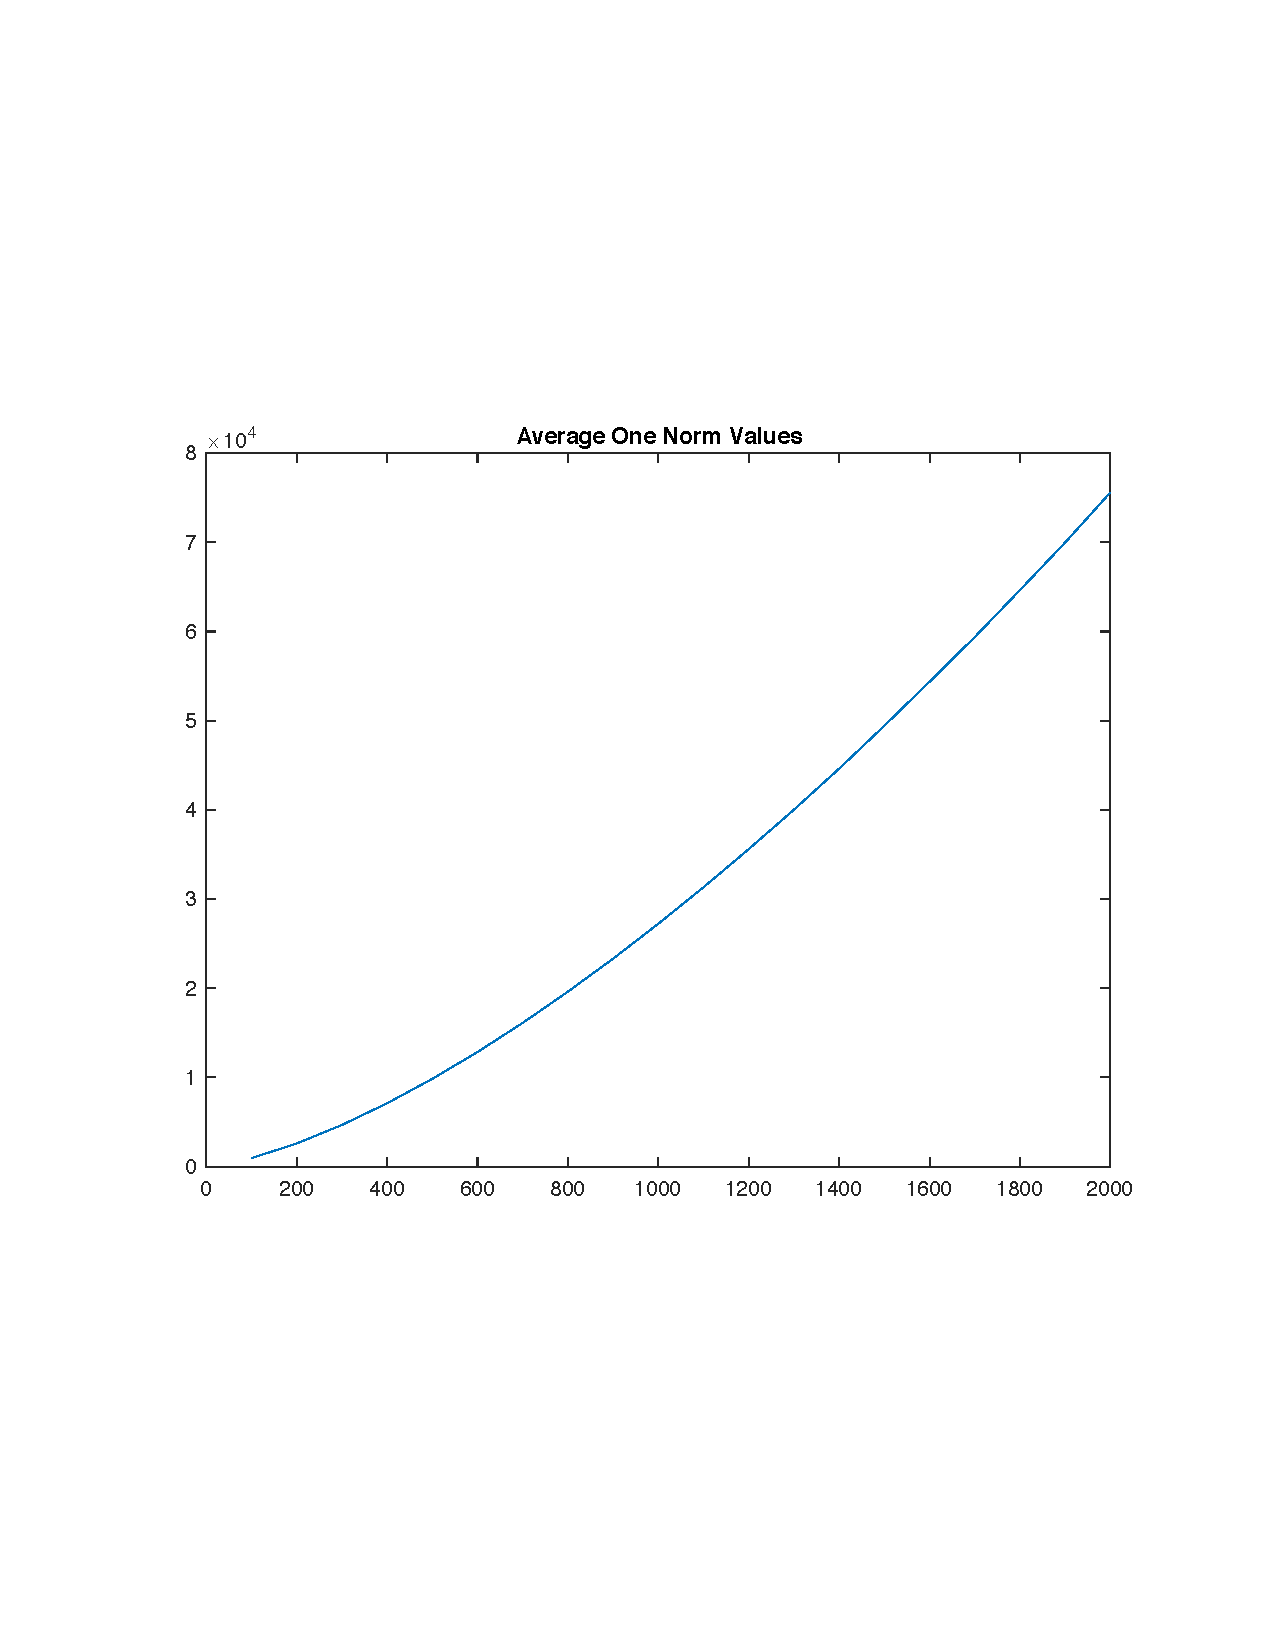
\includegraphics[width=\linewidth]{one}
\end{subfigure}\hspace*{\fill}
\begin{subfigure}{0.48\textwidth}
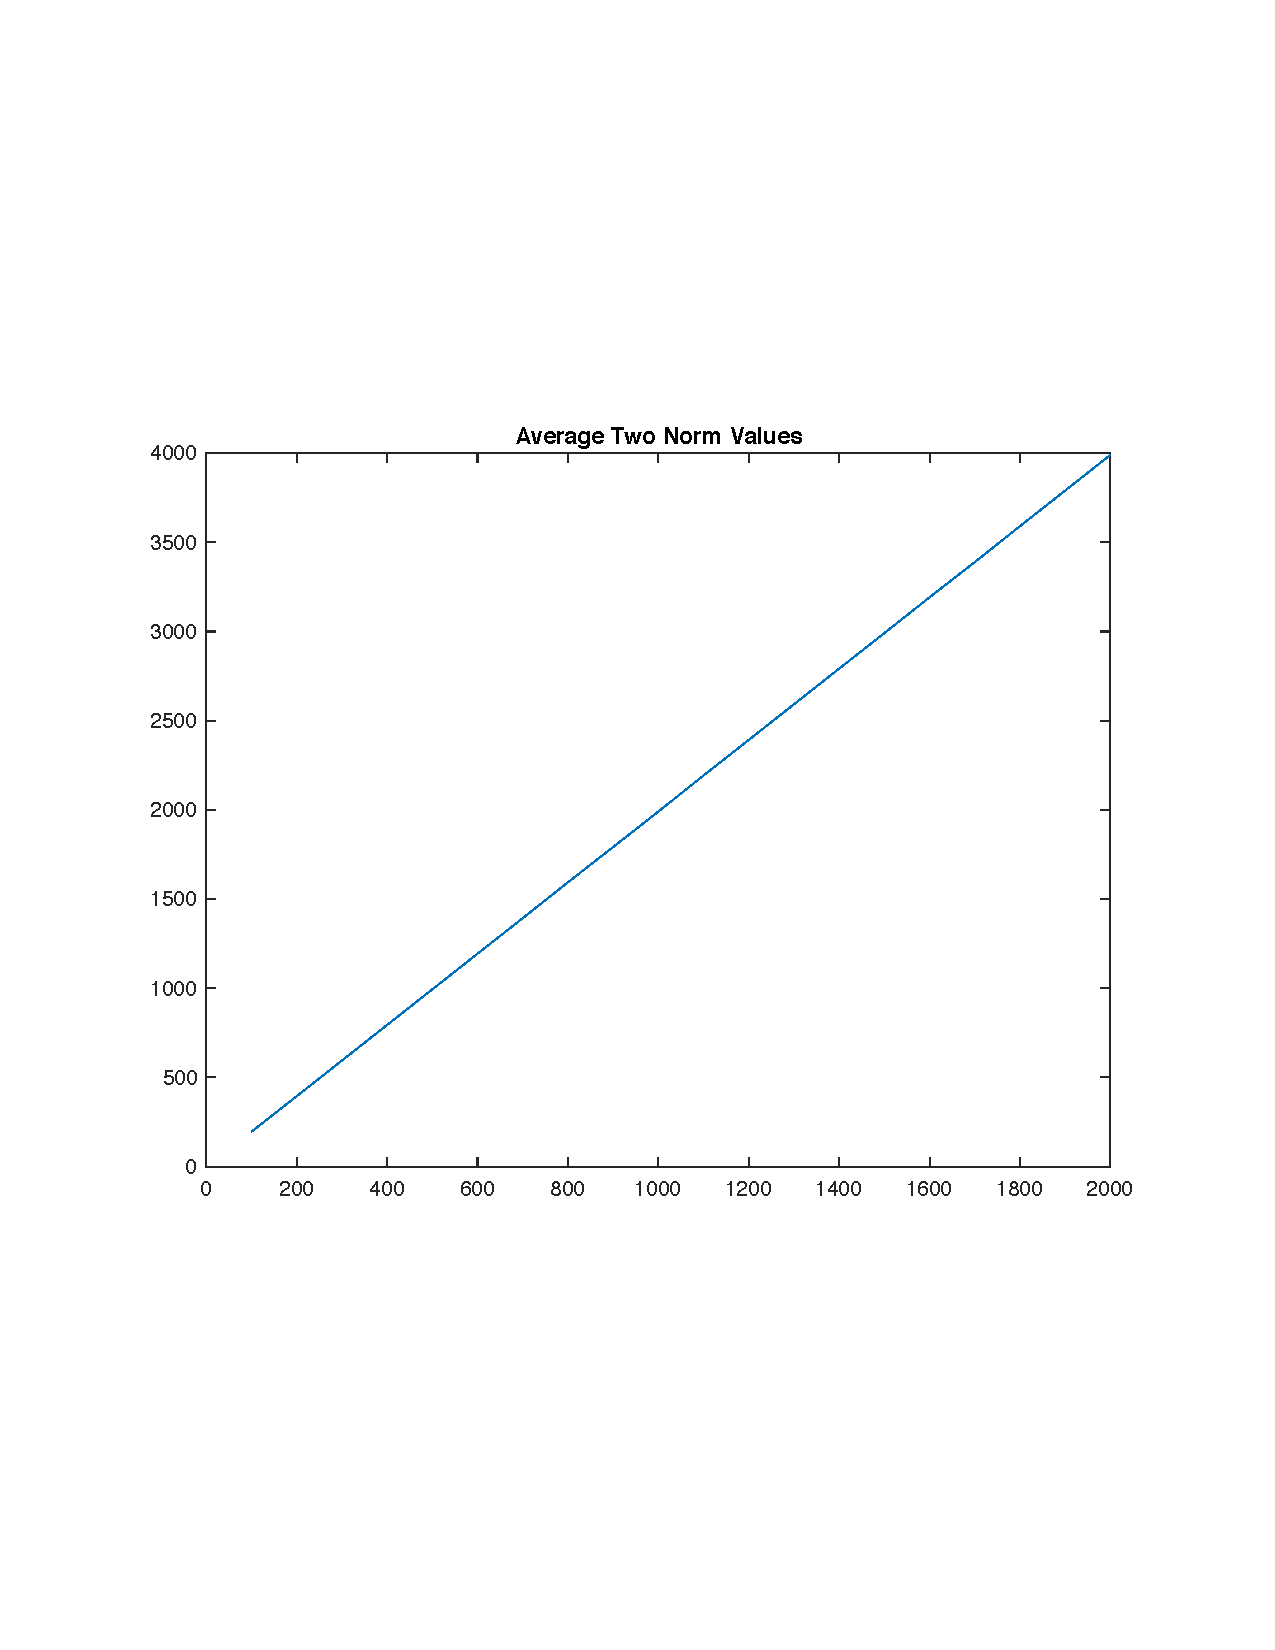
\includegraphics[width=\linewidth]{two}
\end{subfigure}

\begin{subfigure}{0.48\textwidth}
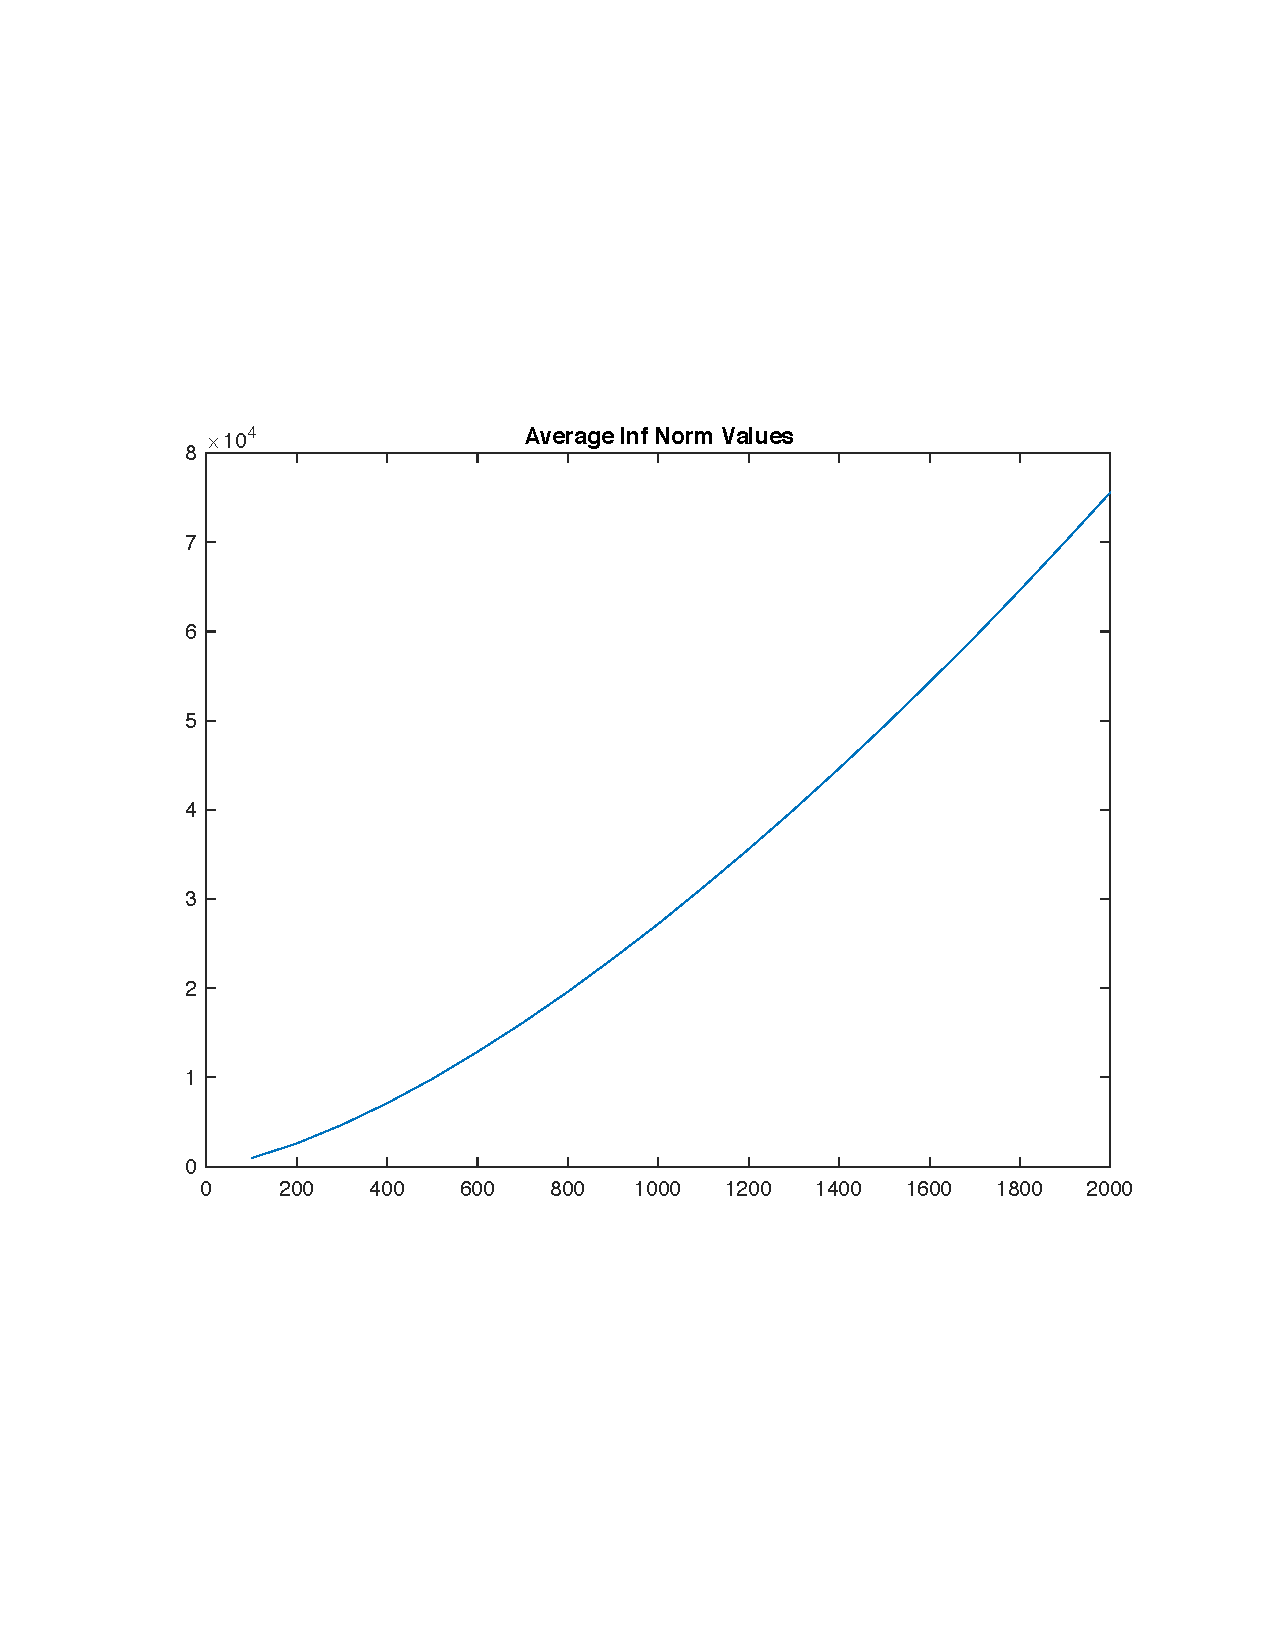
\includegraphics[width=\linewidth]{inf}
\end{subfigure}\hspace*{\fill}
\begin{subfigure}{0.48\textwidth}
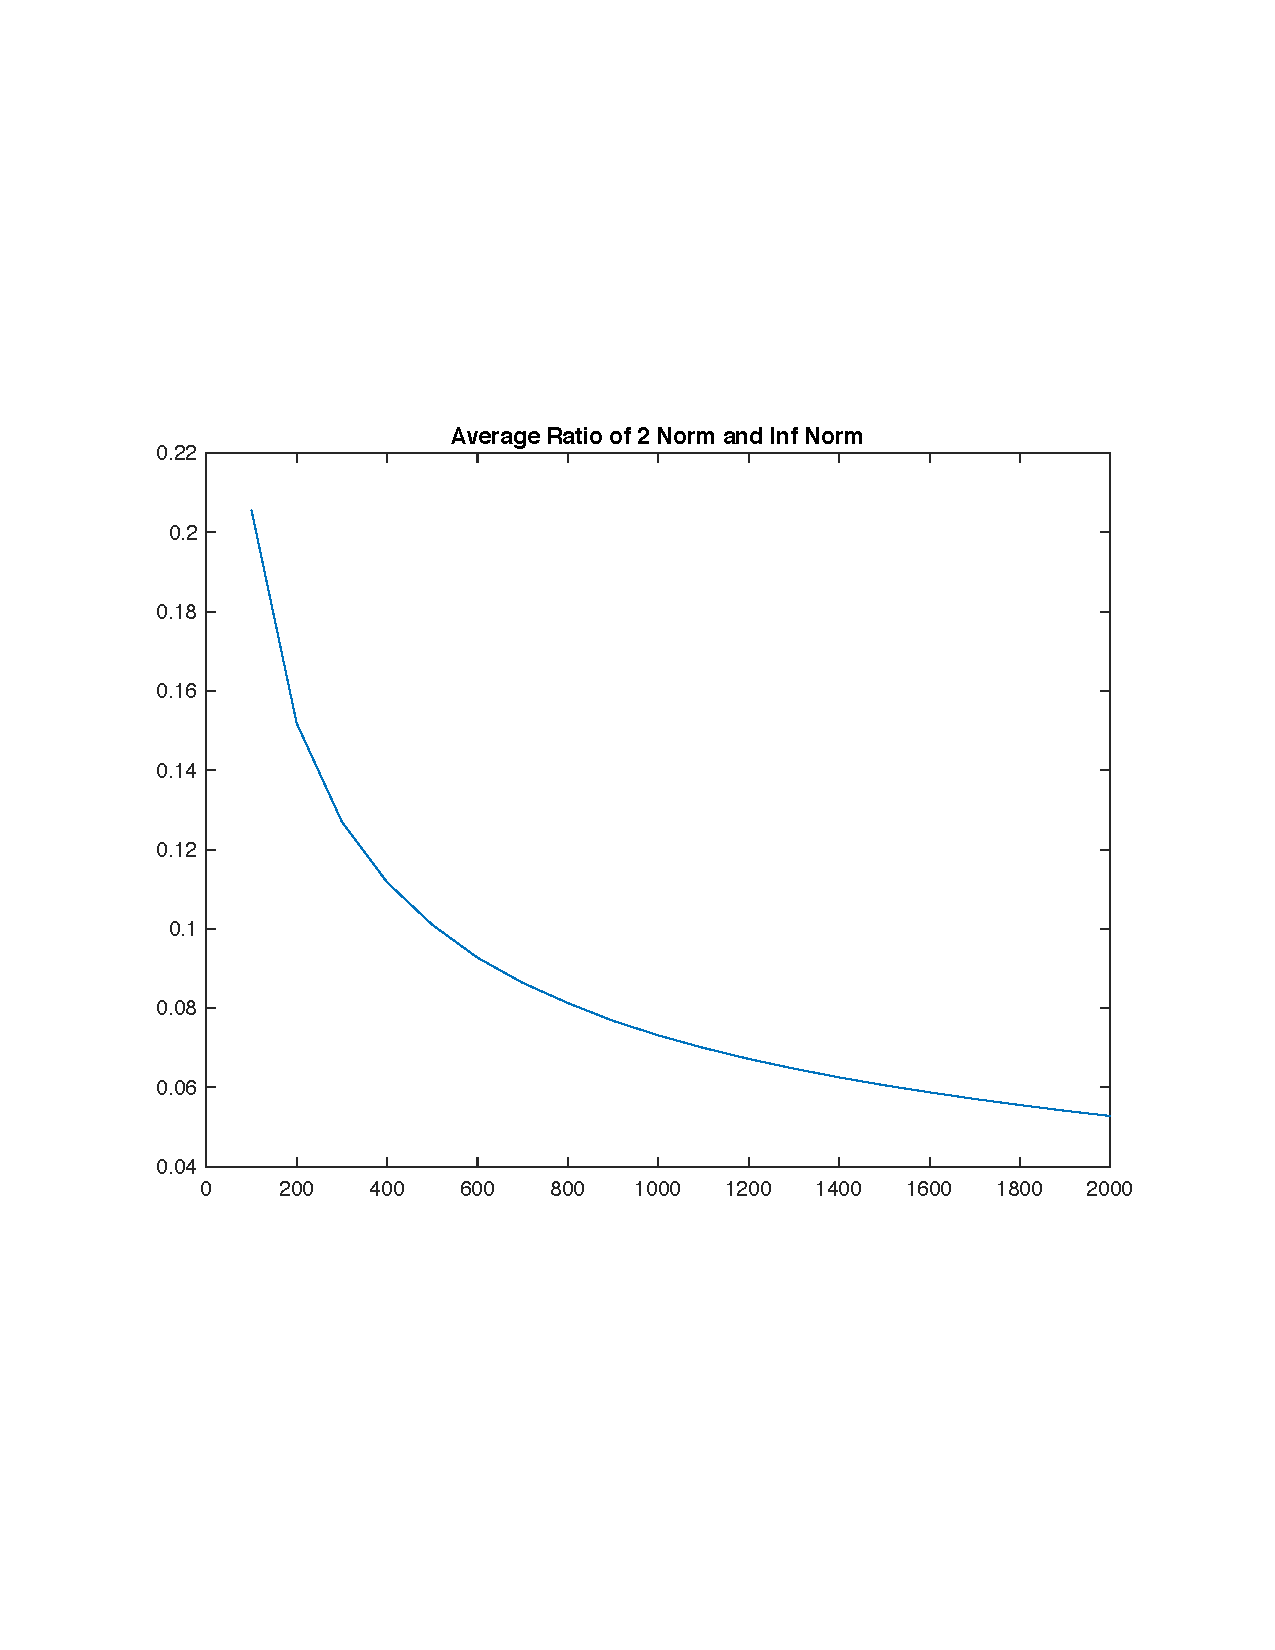
\includegraphics[width=\linewidth]{ratio}
\end{subfigure}

\begin{subfigure}{0.48\textwidth}
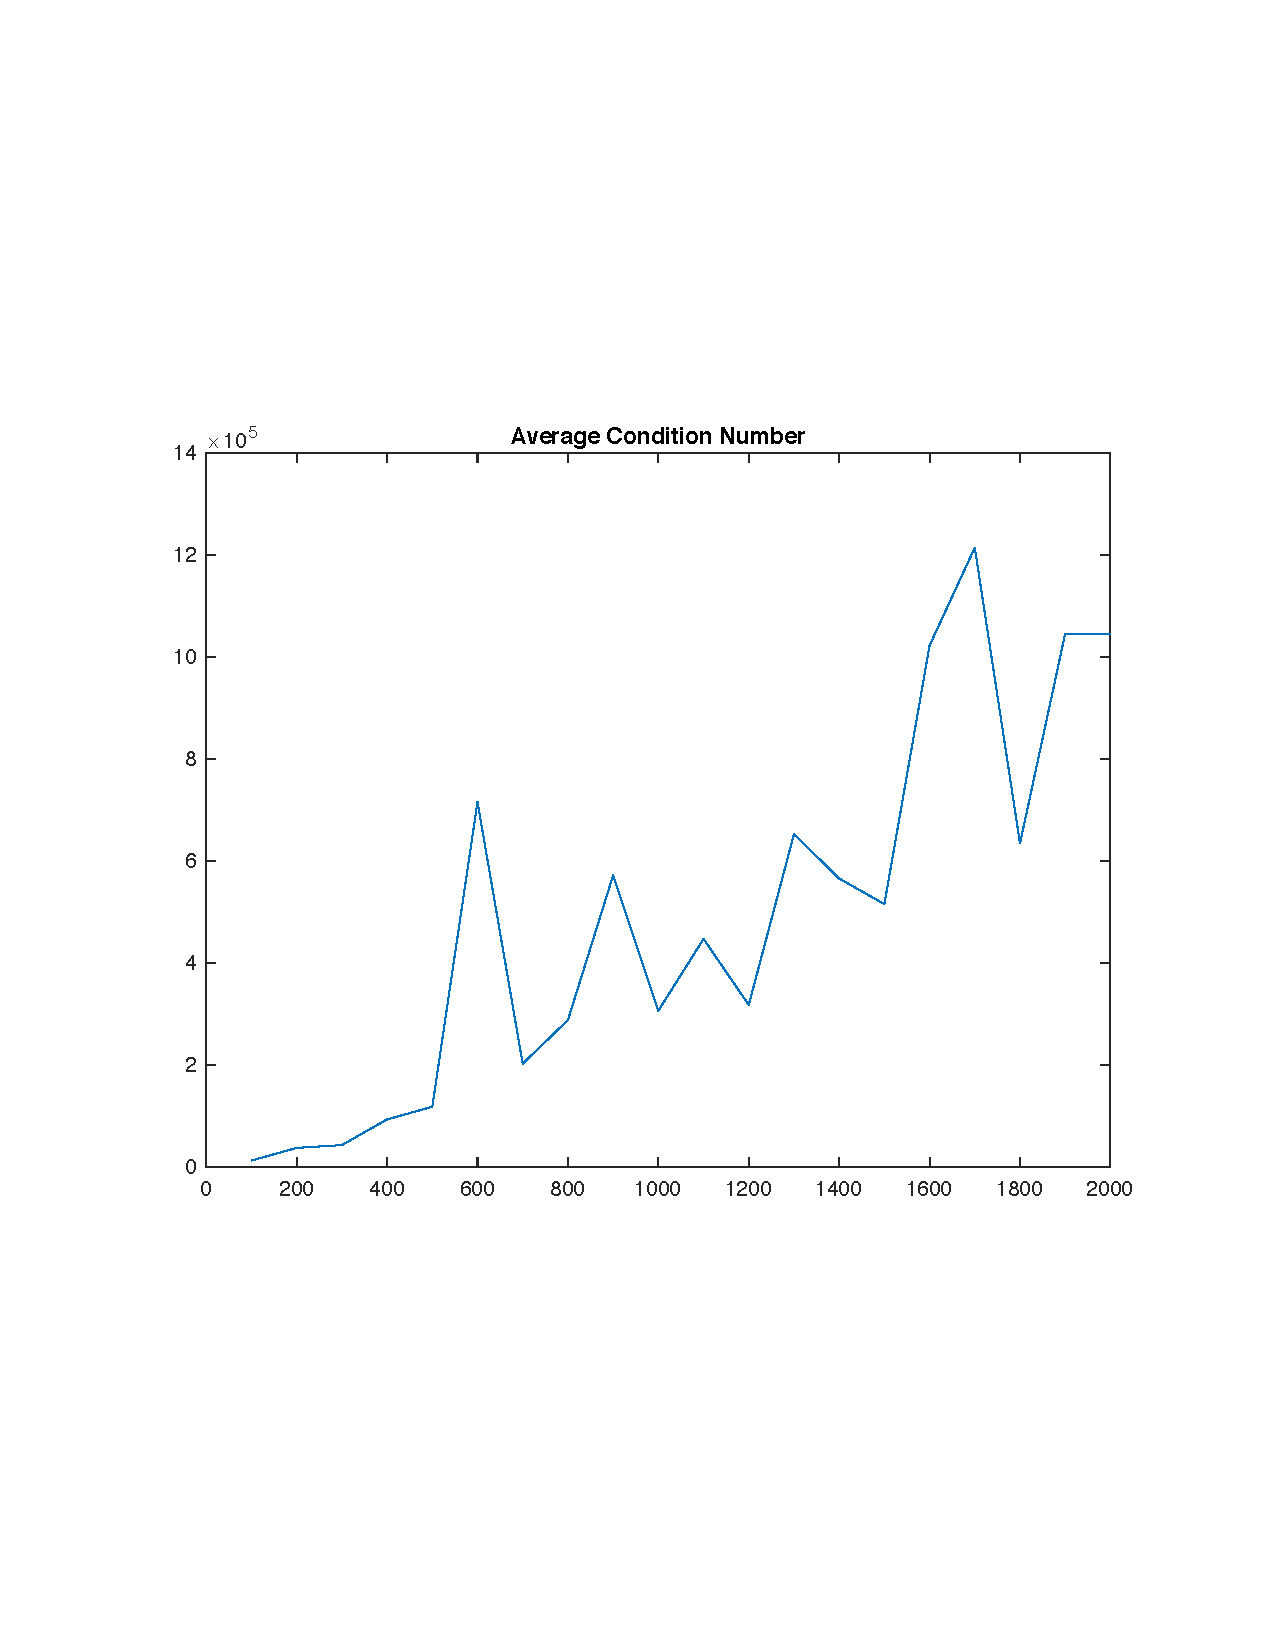
\includegraphics[width=\linewidth]{condition}	
\end{subfigure}

\end{figure}



These results follow intuition, I believe. 
Both the one norm and inf norm can be defined as the maximum of the sum of columns and rows, respectively.
So as $m \to \infty$, it follows that $||A||_1 \to \infty$ and $||A||_{\infty} \to \infty$.
The $||A||_2$ results behave in a more linear manner, which is makes sense given $||A||_2 \ |\lambda_{max}|$. 
Because the two norm behaves linearly and the inf norm behaves super linearly, the ratio between the two should cover to 0 as the inf norm increases at a faster rate.
The condition number for the random matrix overall increases as the size of the matrix increases, though there are dips and spikes in the results.
Overall, this still makes sense as a random matrix will tend to being ill-conditioned as it's size increases. 

\Problem{5}

For this problem, we had to approximate solutions to $-u'' + \lambda u = 3x - \frac{1}{2}$ using Gaussian elimination with and without partial pivoting.
My MATLAB code for this is called ``Problem5''.
My results may be seen in the following graphs:
\begin{figure}[H]
\begin{subfigure}{0.48\textwidth}
\caption{Gaussian elimination for $\lambda = 0$}
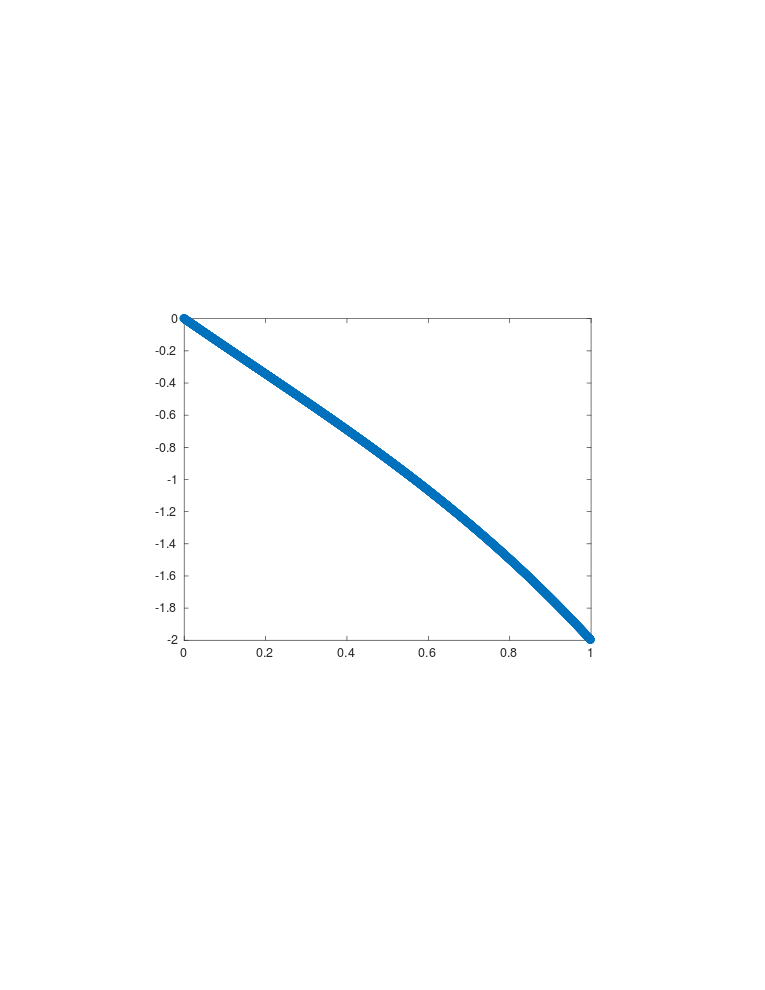
\includegraphics[width=\linewidth]{gaussian_lambda_0_2}
\end{subfigure}\hspace*{\fill}
\begin{subfigure}{0.48\textwidth}
\caption{Gaussian elimination for $\lambda = 2$}
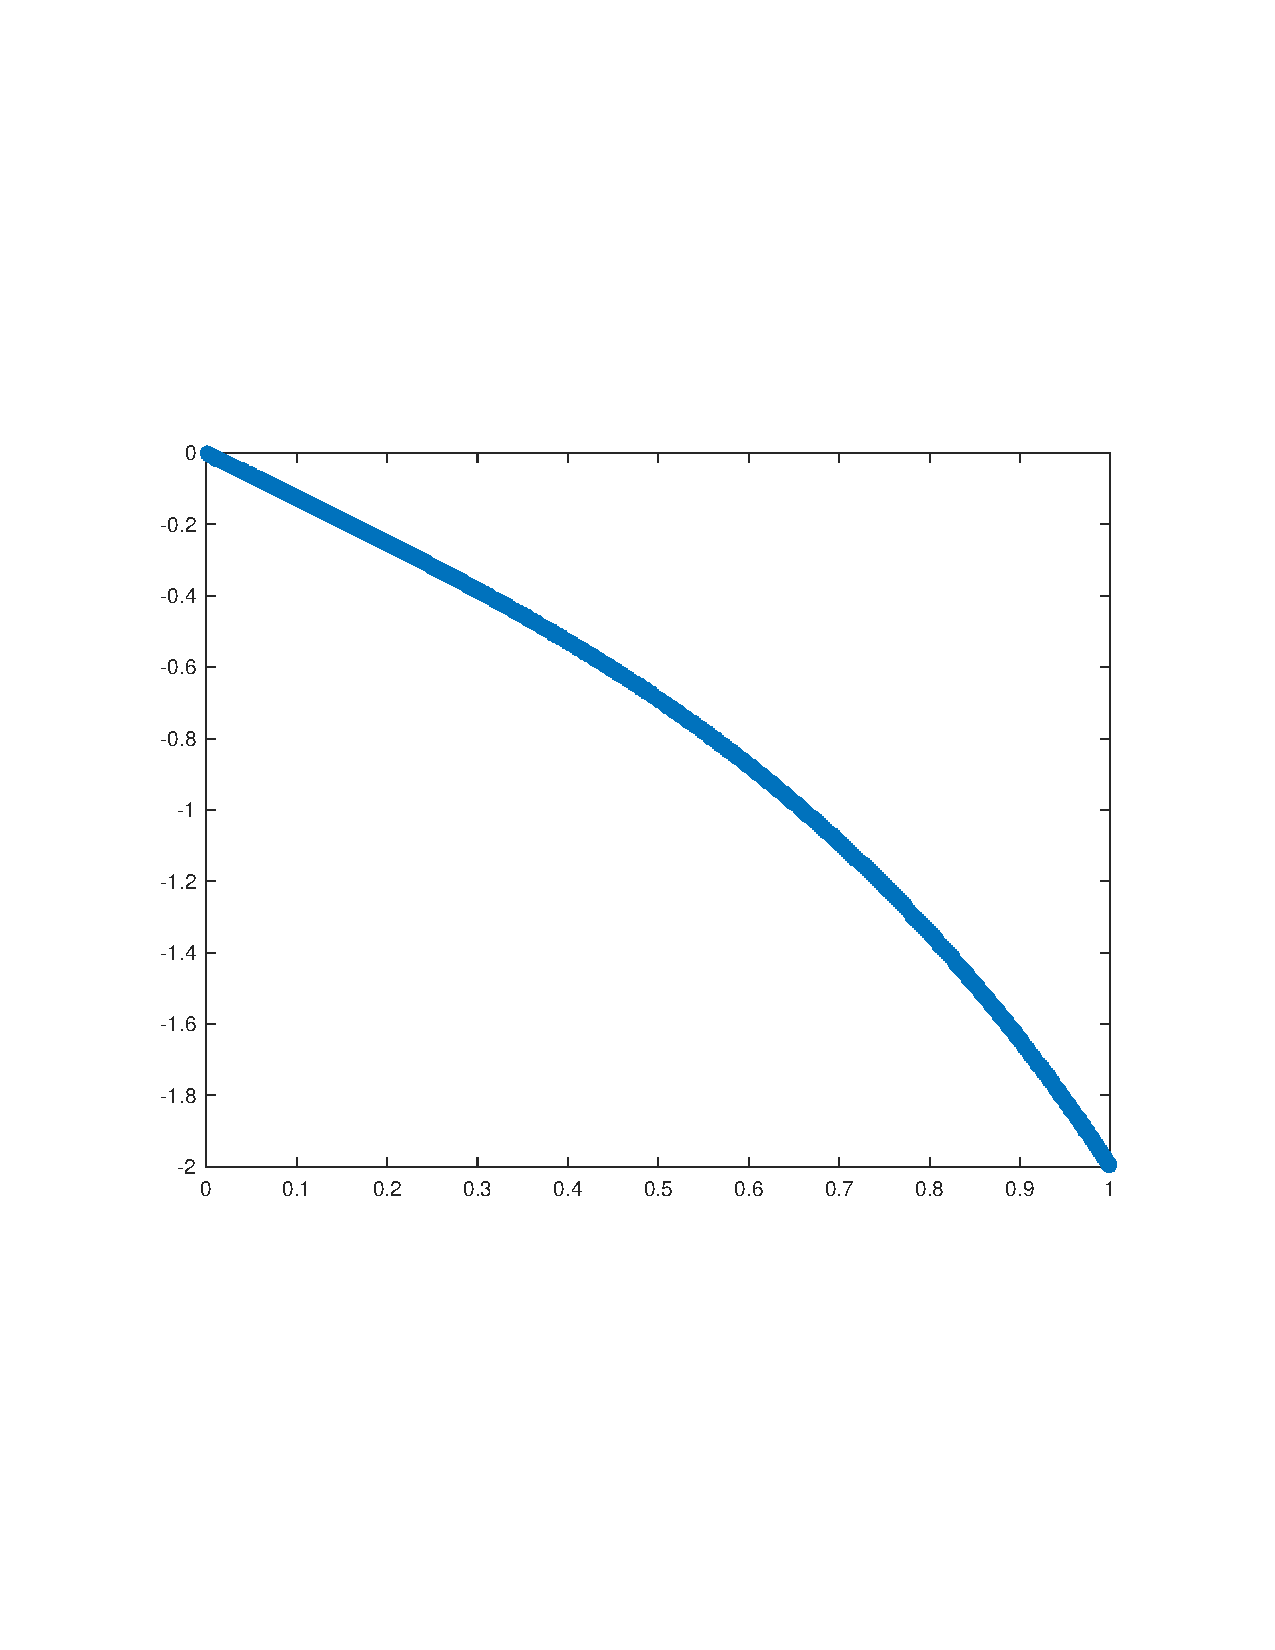
\includegraphics[width=\linewidth]{gaussian_lambda_2}
\end{subfigure}\hspace*{\fill}

\begin{subfigure}{0.48\textwidth}
\caption{True solution for $\lambda = 0$}
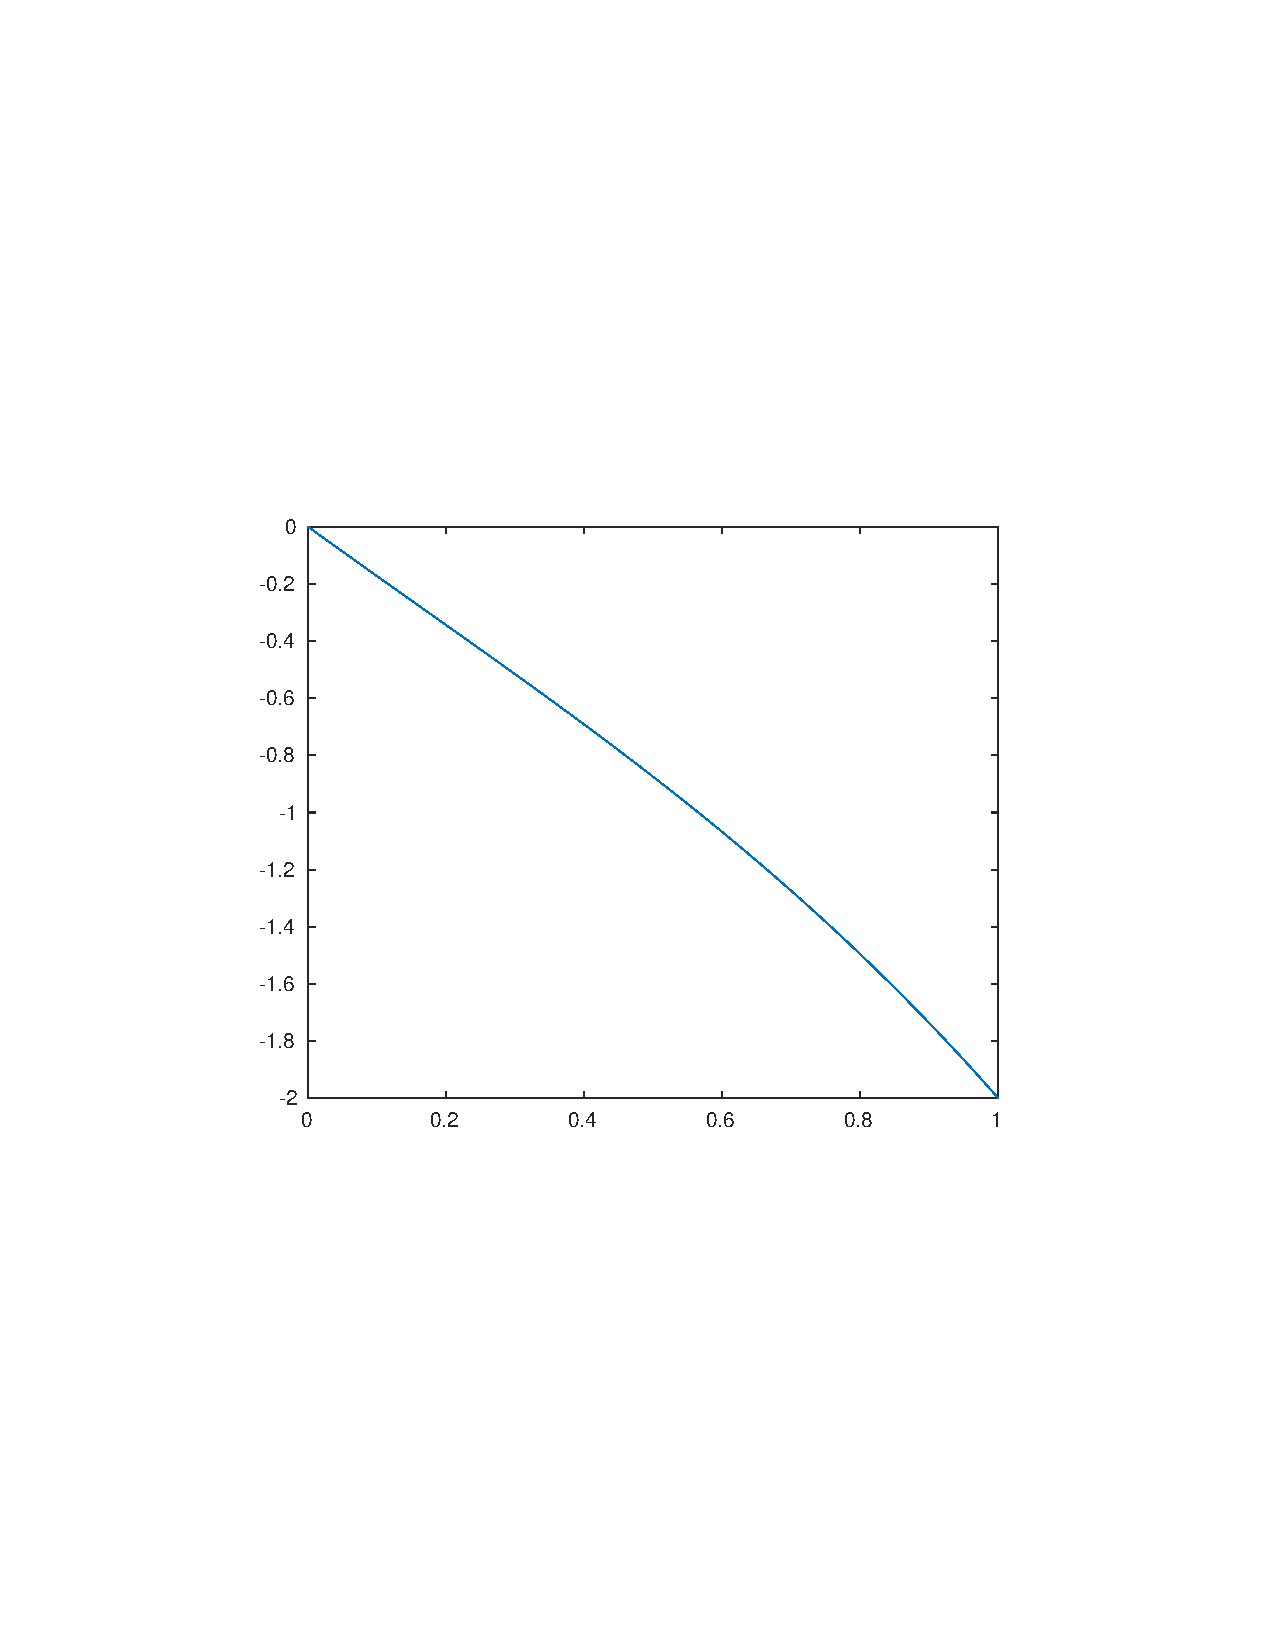
\includegraphics[width=\linewidth]{truesolution_lambda_0}
\end{subfigure}\hspace*{\fill}
\begin{subfigure}{0.48\textwidth}
\caption{True solution for $\lambda = 2$}
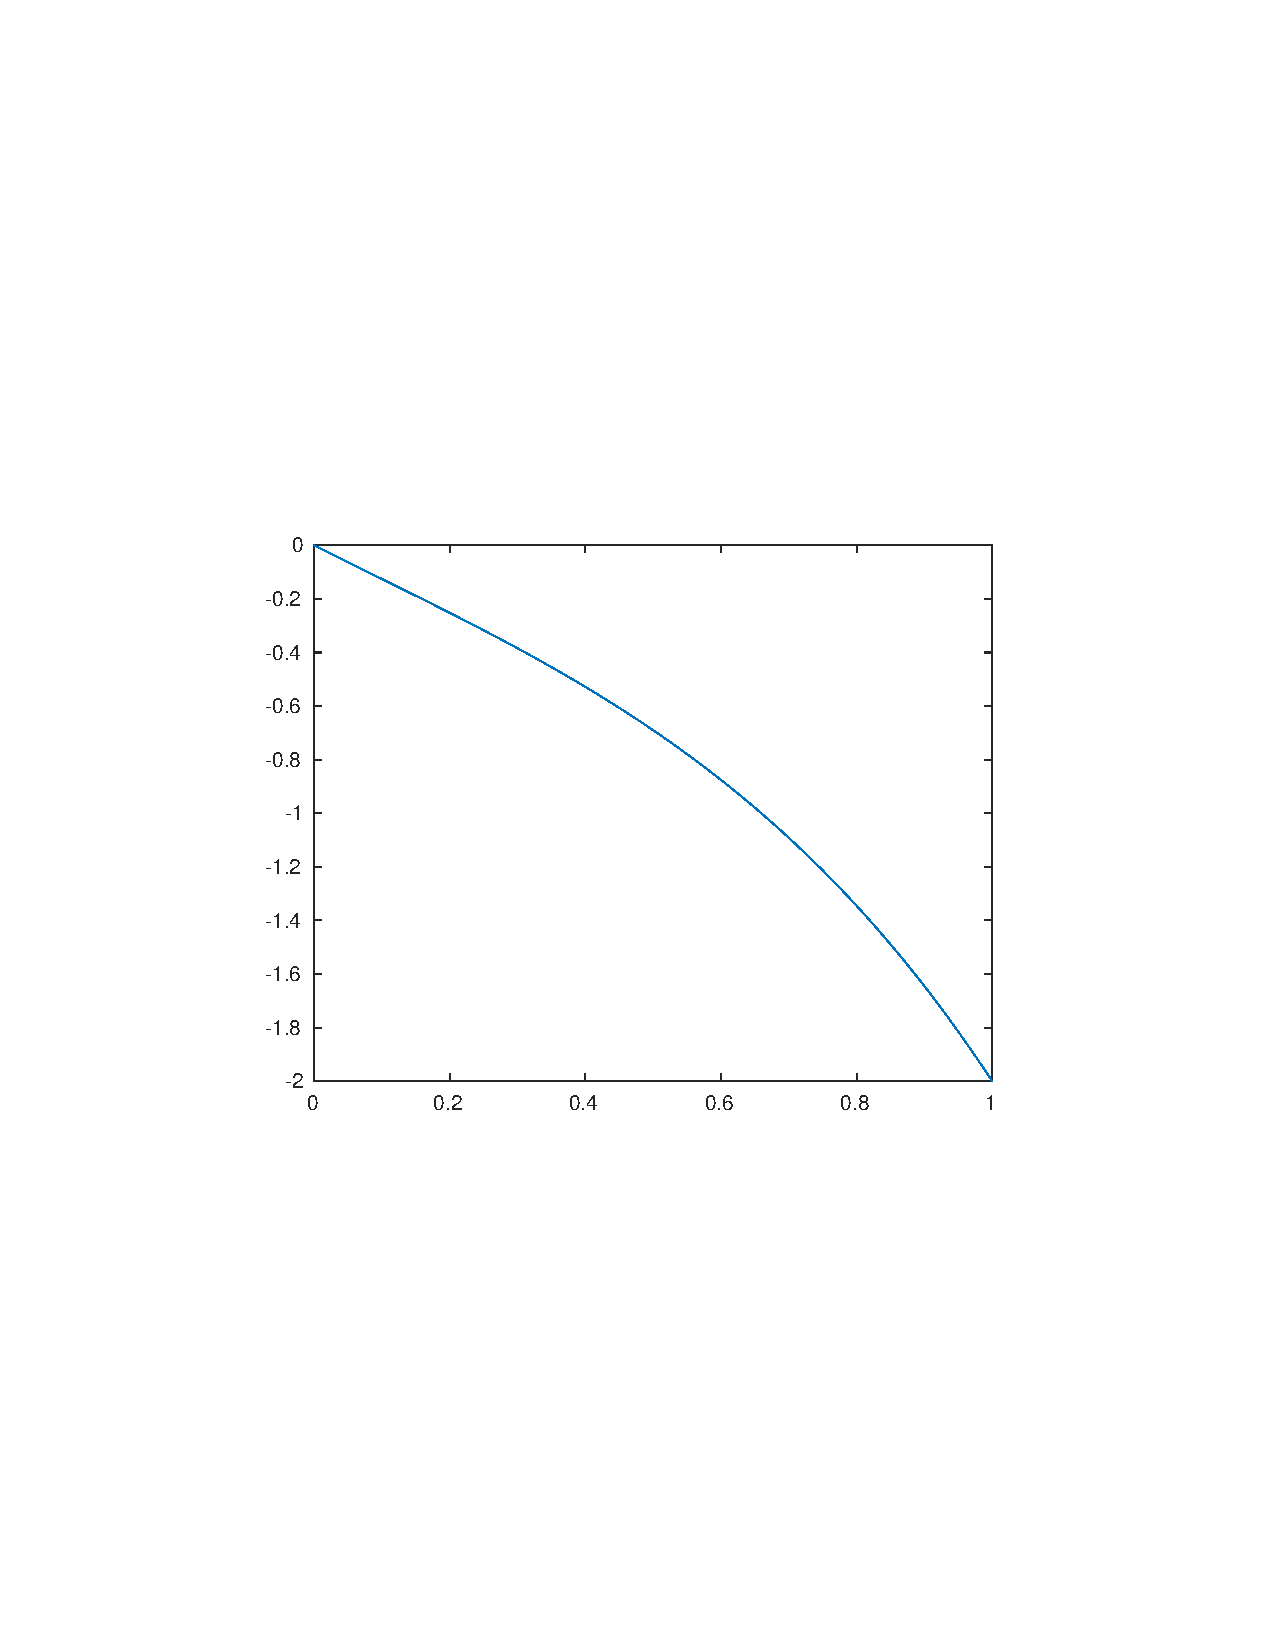
\includegraphics[width=\linewidth]{truesolution_lambda_2}
\end{subfigure}\hspace*{\fill}
\end{figure}

When comparing the true solutions to the differential equation with the approximation, for $\lambda = 0$ the average relative error was on the scale of $10^{-10}$ while for $\lambda = 2$ the average relative error was on the scale of $10^{-16}$.
These are extremely good results, but not surprising as small step sizes were used, which lead to refined answers.
For the various computations, the CPU runtimes are presented below:

\begin{table}[H]
\centering
\caption{CPU Runtimes in seconds}
\begin{tabular}{|l|l|l|l|l|}
\hline
Size & $\lambda = 0$ without pivoting & $\lambda = 0$ with pivoting & $\lambda = 2$ without pivoting & $\lambda = 2$ with pivoting \\
\hline\hline
200 & 0.096323 & 0.264187 & 0.142005 & 0.156812 \\
\hline
400 & 0.300473 & 0.552547 & 0.527399 & 0.421511 \\
\hline
800 & 2.041219 & 3.074913 & 4.295169 & 2.745189 \\
\hline
1000 & 3.963348 & 5.379148 & 8.774305 & 6.098762 \\
\hline
2000 & 34.324527 & 40.059037 & 107.276456 & 85.589778 \\
\hline
4000 & 398.864609 & 313.789217 & 906.203220 & 859.576564\\
\hline
\end{tabular}
\end{table}

These CPU times make sense, as both algorithms theoretically $\sim\frac{2}{3}m^3$ flops.



\end{document}
